% ch16-ml.tex -- Agent patterns
\chapter{Agent patterns}
\label{ch:agents}

Chapters 10--15 treated the model as the system: prompt in, text out,
eval loop around it. This chapter puts the model \emph{inside} a
system that decides what it sees, calls tools on its behalf, and loops
until done --- and asks the question the hype skips: \emph{when is the
loop worth it?} The distinction that organises everything is
Anthropic's~\cite{anthropic_agents}: a \textbf{workflow} is code that
routes an LLM through a fixed path; an \textbf{agent}\index{agent} is
an LLM that chooses its own path. We build both: a prompt chain vs a
monolith, the five workflow patterns as a taxonomy, a 60-line ReAct
agent that works on camera and then fails on camera --- and the eval
harness that scores the trajectories, because an agent without a
trajectory eval is a demo, not a system.

% from-zero:begin
\begin{rulebox}[Before you start]
Chapters~11 and~15. \emph{Recap:} a large language model predicts text. An \emph{agent} wraps it in a loop in which it can call tools and observe results.
\end{rulebox}
\begin{wins}[After this chapter you can]
\begin{itemize}
\item tell a fixed workflow from an agent and choose between them;
\item design the plan--act--observe loop with tools and memory;
\item evaluate an agent by its trajectory, not just its final answer;
\item decide when not to build an agent.
\end{itemize}
\end{wins}
\begin{principle}[How to think about this]
An agent is a language model in a loop with tools. More autonomy means more power and more ways to fail, so use the simplest design that works: a fixed workflow when the steps are known, an agent only when the path really is uncertain. Judge it by what it did, step by step, not just the final sentence.
\end{principle}
% from-zero:end

\section{Workflows vs agents: who controls the path}
\label{sec:wva}

\begin{figure}[htbp]
\centering
\begin{tikzpicture}[font=\scriptsize,
  blk/.style={draw,minimum width=15mm,minimum height=7mm}]
% workflow: code controls
\node[font=\small\bfseries] at (1.8,1.6) {workflow: code controls the path};
\node[blk,fill=amberbg] (q) at (0,0) {input};
\node[blk,fill=accentsoft,right=7mm of q] (m1) {LLM A};
\node[blk,fill=accentsoft,right=7mm of m1] (m2) {LLM B};
\node[blk,fill=amberbg,right=7mm of m2] (out) {output};
\draw[->,thick] (q)--(m1); \draw[->,thick] (m1)--(m2); \draw[->,thick] (m2)--(out);
% agent: model controls
\node[font=\small\bfseries] at (7.9,1.6) {agent: the model decides};
\node[blk,fill=amberbg] (aq) at (6.1,0) {task};
\node[blk,fill=accentsoft,right=8mm of aq] (am) {LLM};
\node[blk,fill=amberbg,below=6mm of am] (tool) {tool / env};
\draw[->,thick] (aq)--(am);
\draw[->,thick] (am)-- node[right]{\scriptsize action} (tool);
\draw[->,thick] (tool.west) .. controls (6.5,-0.9) .. node[below]{\scriptsize observation} (am.south);
\end{tikzpicture}
\caption{The whole distinction in two boxes. Left: a fixed pipeline
--- the code's flowchart is the architecture; the LLM fills slots.
Right: a loop --- the model picks the next action; code only
executes it.}
\label{fig:wva}
\end{figure}

The workflow is debuggable, testable, and boring --- which is why it
ships. The agent can handle the inputs no flowchart anticipated ---
which is why it loops, wanders, and costs tokens you didn't plan.
Choose the workflow unless the task's decision tree is too large or
too ambiguous to write down~\cite{anthropic_agents}; most
``agentic'' products are three workflows and a retrieval call.

\section{The augmented LLM: the building block}
\label{sec:aug}

Everything in this chapter is composed of one unit: an LLM plus
attachments --- \emph{retrieval} (documents fetched into context),
\emph{tools} (schemas it can call: calculator, search, code),
and \emph{memory} (state carried across calls). The attachments are
what make it a \emph{system}: the base model only completes text.
Chapter 11's attention is the engine; this chapter is the chassis.

\section{The five workflow patterns}
\label{sec:patterns}

\begin{itemize}
\item \textbf{Prompt chaining}: decompose into a fixed sequence ---
extract, then answer, then format --- each step checkable and
replaceable. The listing below is the smallest real one.
\item \textbf{Routing}: a cheap classifier (often an LLM) sends each
input to a specialist path --- triage tickets to billing/tech/legal
models rather than one giant prompt.
\item \textbf{Parallelisation}: run subtasks concurrently ---
independent extractions, or vote among $k$ samples of the same call.
\item \textbf{Orchestrator--workers}: an LLM decomposes the task,
farms subtasks to worker calls, and joins the results --- the
workhorse of research/report tasks.
\item \textbf{Evaluator--optimiser}: generate, grade against a
rubric (ch15's own instrument), loop until the grade clears a bar or
the budget dies.
\end{itemize}

\begin{figure}[htbp]
\centering
\begin{tikzpicture}[font=\scriptsize,x=8mm,y=8mm,
  blk/.style={draw,minimum width=8mm,minimum height=5mm}]
% chaining
\node[font=\scriptsize\bfseries] at (1.5,1.4) {chaining};
\foreach \x in {0,1.2,2.4} \node[blk,fill=accentsoft] at (\x,0.6) {};
\draw[->](0.5,0.6)--(0.7,0.6); \draw[->](1.7,0.6)--(1.9,0.6);
% routing
\node[font=\scriptsize\bfseries] at (4.9,1.4) {routing};
\node[blk,fill=amberbg] (r) at (4.9,0.6) {};
\node[blk,fill=accentsoft] (r1) at (4.2,-0.5) {}; \node[blk,fill=accentsoft] (r2) at (5.6,-0.5) {};
\draw[->](r)--(r1); \draw[->](r)--(r2);
% parallel
\node[font=\scriptsize\bfseries] at (8.2,1.4) {parallel};
\node[blk,fill=amberbg] (p) at (8.2,0.9) {};
\node[blk,fill=accentsoft] (p1) at (7.6,0) {}; \node[blk,fill=accentsoft] (p2) at (8.8,0) {};
\node[blk,fill=amberbg] (pj) at (8.2,-0.9) {};
\draw[->](p)--(p1); \draw[->](p)--(p2); \draw[->](p1)--(pj); \draw[->](p2)--(pj);
% orchestrator
\node[font=\scriptsize\bfseries] at (11.2,1.4) {orchestrator};
\node[blk,fill=amberbg] (o) at (11.2,0.9) {};
\node[blk,fill=accentsoft] (o1) at (10.6,0) {}; \node[blk,fill=accentsoft] (o2) at (11.8,0) {};
\node[blk,fill=amberbg] (oj) at (11.2,-0.9) {};
\draw[->](o)--(o1); \draw[->](o)--(o2); \draw[->](o1)--(oj); \draw[->](o2)--(oj);
% evaluator
\node[font=\scriptsize\bfseries] at (14.0,1.4) {eval-opt};
\node[blk,fill=accentsoft] (g) at (13.7,0.6) {gen};
\node[blk,fill=amberbg] (e) at (15.0,-0.4) {eval};
\draw[->,bend left=25] (g) to (e); \draw[->,bend left=25] (e) to node[above]{\scriptsize retry} (g);
\end{tikzpicture}
\caption{The five workflow patterns as shapes: fixed pipelines, a
switch, a fan-out/join, a decomposer/join, and a grade-retry loop.}
\label{fig:patterns}
\end{figure}

\lstinputlisting[language=Python,caption={\texttt{prompt\_chain.py}: the same question via a two-step chain vs one monolithic prompt, on a good and a weak mock LLM --- the control-vs-latency trade in three lines of output.},label=lst:chain]{code/ch16/prompt_chain.py}

\lstinputlisting[numbers=none]{code/ch16/prompt_chain.out.txt}

\begin{example}[WE 16.1 --- 2 calls vs 1: what chaining buys]
\label{ex:chain}
On the good model both paths answer; the difference is \emph{where}
they can fail. The chain's extract step prints
\texttt{41.2,38.7,4.5,1204} --- inspectable, fixable, replaceable ---
before the answer step ever runs. On the weak model the monolith
collapses to ``I am unsure, the text contains many numbers'' while
the chain still answers (the extract step carries the load). Chain
when the sub-steps have different failure modes or need different
models; stay monolithic when the task is one thought and latency is
the metric.
\end{example}

\section{Agents: the plan--act--observe loop}
\label{sec:react}

A minimal agent is a loop: the model emits \emph{Thought} +
\emph{Action} (a tool call) or \emph{Final}; the code executes the
tool, appends the \emph{Observation}, and re-asks --- the
ReAct~\cite{react} loop in 60 lines.

\lstinputlisting[language=Python,caption={\texttt{code/ch16/react\_minimal.py}: the loop, two tools (calculator, mock search), a loop-detector, and a trace dump --- plus the injected tool error that makes it fail on camera.},label=lst:react]{code/ch16/react_minimal.py}

\lstinputlisting[numbers=none]{code/ch16/react_minimal.out.txt}

\begin{example}[WE 16.2 --- 3 steps to 37.50; then 8 identical failures]
\label{ex:react}
The success trace is the textbook picture:
\texttt{search(unit price)} $\to$ \texttt{12.50} $\to$
\texttt{calc(3*12.50)} $\to$ \texttt{37.5} $\to$ \texttt{Final: 37.50}.
Then the tool-error run: the model retries the \emph{identical}
search call eight times --- the loop-detector's duplicate-check and
\texttt{max\_steps=8} are the only things between it and an unbounded
retry storm. That is the failure catalogue in one trace: no
perception that the observation changed nothing (it never re-reads
the result), no alternative plan, no budget awareness. The fixes are
mechanical --- deduplicate actions, cap iterations, surface the error
in context --- and the lesson is that agents fail \emph{at the loop},
not at the model.
\end{example}

\begin{figure}[htbp]
\centering
\begin{minipage}[t]{0.55\linewidth}
\centering
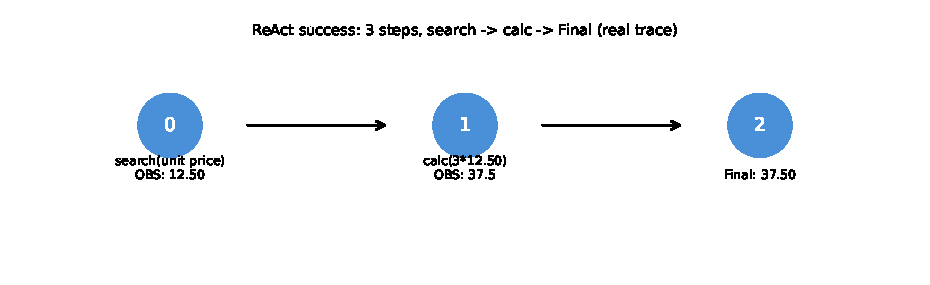
\includegraphics[width=\linewidth]{figures/ch16/react_trace.pdf}
\caption{The success trace as a timeline --- three decisions, two
tools, one answer.}
\label{fig:react}
\end{minipage}\hfill
\begin{minipage}[t]{0.42\linewidth}
\centering
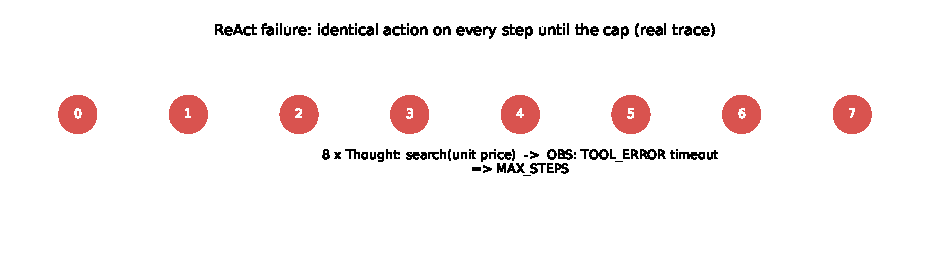
\includegraphics[width=\linewidth]{figures/ch16/fail_trace.pdf}
\caption{The failure trace: the same action 8 times --- a loop, not
a plan.}
\label{fig:fail}
\end{minipage}
\end{figure}

\section{Memory and tool use}
\label{sec:memtool}

\textbf{Memory} splits by horizon: the context window is working
memory (expensive, fast, wiped each call); a scratchpad is
task-scoped state (the trace itself is ours); and \emph{retrieval
memory} stores distilled facts to re-inject later --- the design
question is what to \emph{store} (facts, not transcripts) and how to
fetch it (recency + relevance, not a dump). \textbf{Tool use} is a
contract, not a capability: each tool needs a schema the model can
read, an error surface it can react to (ours prints
\texttt{TOOL\_ERROR}/\texttt{CALC\_ERROR}), and a cost the loop
budgets for. Toolformer~\cite{toolformer} showed models can learn
tool calls; our listing shows the contract must be enforced in code
--- the model emits the call, the code decides if it runs.

\section{Evaluating agents: trajectories, not outputs}
\label{sec:agenteval}

ch15's eval loop generalises: the artifact to score is the
\emph{trajectory} --- steps taken, tools called, errors hit, tokens
spent --- because two runs that print the same answer can have wildly
different efficiency and risk.

\lstinputlisting[language=Python,caption={\texttt{code/ch16/agent\_eval.py}: an 8-run battery scored on success, steps, tool errors and cost --- and the honest note that step-count alone won't catch a wrong early Final.},label=lst:eval]{code/ch16/agent_eval.py}

\lstinputlisting[numbers=none]{code/ch16/agent_eval.out.txt}

\begin{example}[WE 16.3 --- 62\% success and the run the table misses]
\label{ex:agenteval}
The battery reads: 5/8 success, mean 5.4 steps, 2 loop-terminations
(both failures), \$0.0016/run but \$0.0026 per success --- cost
belongs \emph{per success}, not per call. And the printed caveat is
the deep lesson: run 8 terminated in 2 steps at \$0.0004 ---
the \emph{cheapest} run --- by calling Final early with a wrong
answer. Step-count and cost both reward it; only an outcome check
convicts it. Agent evals need the trajectory \emph{and} the result:
rate the path, verify the destination.
\end{example}

\begin{figure}[htbp]
\centering
\begin{minipage}[t]{0.56\linewidth}
\centering
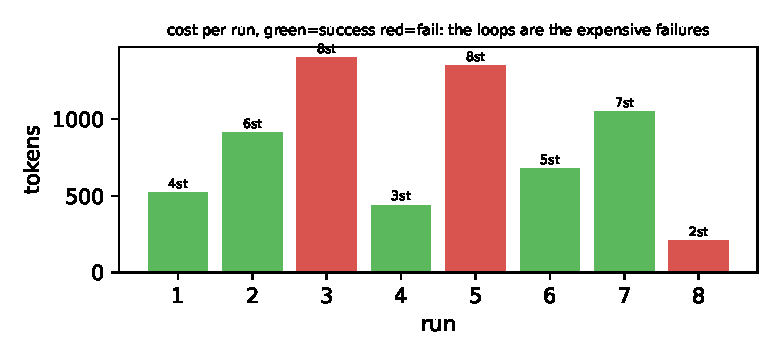
\includegraphics[width=\linewidth]{figures/ch16/agent_eval_cost.pdf}
\caption{Cost per run: the two 8-step loops are the expensive
failures; the cheap failure is the dangerous one.}
\label{fig:evalcost}
\end{minipage}\hfill
\begin{minipage}[t]{0.4\linewidth}
\centering
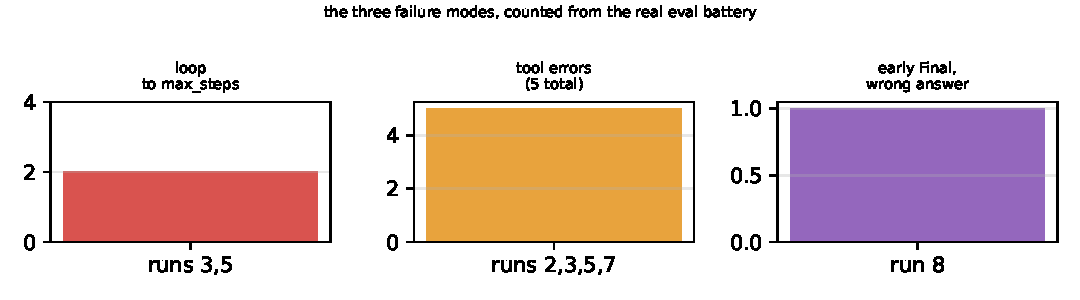
\includegraphics[width=\linewidth]{figures/ch16/failure_gallery.pdf}
\caption{The three failure modes, counted: loops, tool errors,
early-Final.}
\label{fig:failgal}
\end{minipage}
\end{figure}

\begin{figure}[htbp]
\centering
\begin{minipage}[t]{0.52\linewidth}
\centering
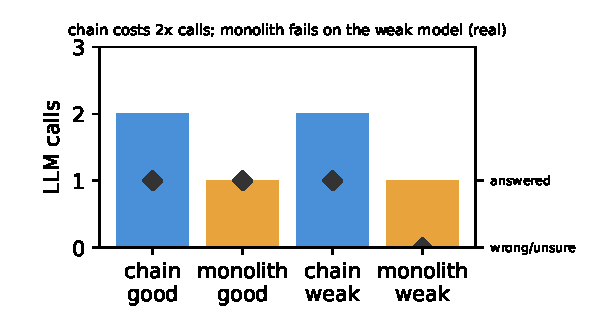
\includegraphics[width=\linewidth]{figures/ch16/chain_compare.pdf}
\caption{Chaining doubles calls but survives the weak model; the
monolith is cheaper until it isn't.}
\label{fig:chaincmp}
\end{minipage}\hfill
\begin{minipage}[t]{0.44\linewidth}
\centering
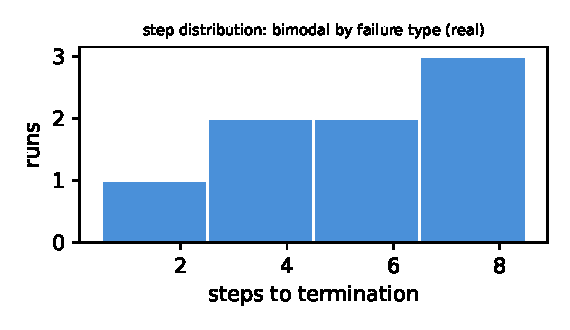
\includegraphics[width=\linewidth]{figures/ch16/steps_hist.pdf}
\caption{Step distribution: the failures cluster at the loop cap ---
bimodal by design.}
\label{fig:steps}
\end{minipage}
\end{figure}

\section{When NOT to build an agent}
\label{sec:noagent}

The honest checklist~\cite{anthropic_agents}: build a workflow when
the decision tree is enumerable, when a wrong path costs more than a
missed shortcut, when the task is high-volume/low-value (agents burn
tokens exploring), and when you can't write the eval that would catch
a wandering run. Build an agent when the task is ambiguous and
valuable, when the search space is too wide to script, and when you
have the eval harness to watch it. The framework landscape
(LangChain, HF agents course~\cite{langchain,hf_agents}) implements
these same patterns [checked 2026-10]; the decision is older than any
framework~\cite{wiki_agent}.

\section{Common mistakes}
\label{sec:agentmistakes}

\begin{description}
\item[No loop budget] Our trace needed \texttt{max\_steps} and a
duplicate-action detector to terminate at all --- an agent without
both is a while(True) on your API key.
\item[Tools with vague contracts] ``search'' that can return anything
teaches the model to retry blindly; schemas + typed errors are what
make actions legible.
\item[Evaluating the answer, not the trajectory] Run 8 answered cheap
and wrong --- score the path and the outcome separately.
\item[Retrieval as a dump] Stuffing whole transcripts into memory
spends context on noise; store distilled facts, fetch by relevance.
\item[One model for every step] The extract/routing/grading steps are
cheap-model jobs; paying flagship prices per slot is the default
mistake.
\item[Agents for workflow-shaped tasks] If the flowchart fits on a
napkin, the code that draws it will beat the loop that guesses it.
\end{description}

\begin{example}[WE 16.4 --- Cost arithmetic: per-run vs per-success]
\label{ex:cost}
The battery spends \$0.0128 across 8 runs (mean \$0.0016) for 5
successes. Cost-per-success is \$0.0026 --- $1.6\times$ the
per-run figure, because failures still burn tokens. Scale it: at 10k
tasks/day the gap is \$16 vs \$26 daily --- the number that matters
for budgeting is always per-\emph{success}, and it rises exactly as
success rate falls. An agent that costs \$0.001/run at 60\% success
is \$0.0017/outcome --- the denominator is the product.
\end{example}
\begin{example}[WE 16.5 --- What the loop-detector actually sees]
\label{ex:loopdet}
Step 3 of the failure trace: the context holds
\texttt{search(unit price)} three times. The dedup check hashes
(action, args) and finds the pair already in \texttt{seen} --- it
fires not on \emph{time} or \emph{count} but on \emph{identity}:
repeating the exact call. That distinction is the design: a
legitimate agent may search twice with different queries, and a dumb
one may alternate two actions forever (ABABABA). Identity dedup
catches the first; only the no-progress variant catches the second
--- which is why the honest guard is two checks, not one.
\end{example}

\section{Summary table}
\label{sec:agentsummary}

\begin{center}\small
\begin{tabular}{p{3.0cm}p{3.2cm}p{3.0cm}p{3.0cm}}
\toprule
pattern & when it wins & cost & failure mode \\
\midrule
prompt chain & separable sub-steps & 1 call/step, predictable & error compounding down the chain \\
routing & heterogeneous inputs & cheap classifier + one call & misroutes to the wrong specialist \\
parallelisation & independent subtasks & $k$ calls at once & join conflicts; $k\times$ cost \\
orchestrator--workers & decomposable research & $1 + \sum$ workers & bad decomposition poisons all workers \\
evaluator--optimiser & gradable outputs & gen+eval per round & loop until budget or bar --- unbounded \\
ReAct agent & ambiguous, valuable tasks & unbounded by default & loops, tool misuse, context overflow \\
\bottomrule
\end{tabular}
\end{center}

The meta-rule: \emph{every step up this table buys flexibility by
spending control}. Spend control only on tasks that pay for it.

\section*{Drill}
\begin{enumerate}
\item Workflow or agent: a pipeline that formats invoices into JSON
--- and a research assistant that must plan its own searches?
\item In our ReAct trace, what two code-level guards stopped the
infinite retry?
\item Why is ``\$0.0016 per run'' a misleading cost figure --- what
should it be divided by?
\item Name the three failure modes our eval battery counted, and
which one escapes step-count metrics.
\item What goes in \emph{retrieval} memory vs the context window?
\end{enumerate}

\section*{Further reading}
\label{sec:further16}
\begin{itemize}
\item Anthropic, \emph{Building effective agents} (2024) --- the
workflow/agent distinction and the ``when not to'' checklist this
chapter borrows.
\url{https://www.anthropic.com/research/building-effective-agents}
\item Yao et al., \emph{ReAct} (ICLR 2023) --- the Thought/Action/
Observation loop our 60 lines implement.
\url{https://arxiv.org/abs/2210.03629}
\item Schick et al., \emph{Toolformer} (2023) --- models learning to
call tools; the origin of the tool-use contract idea.
\url{https://arxiv.org/abs/2302.04761}
\item LangChain \emph{Concepts} docs --- the framework version of
these same patterns [checked 2026-10].
\url{https://python.langchain.com/docs/concepts/}
\item Hugging Face, \emph{Agents course: what are agents} --- a free
course with runnable agent exercises.
\url{https://huggingface.co/learn/agents-course/en/unit1/what-are-agents}
\item Wikipedia, \emph{Intelligent agent} --- the pre-LLM intellectual
lineage (BDI, control loops).
\url{https://en.wikipedia.org/wiki/Intelligent_agent}
\end{itemize}

\begin{rulebox}[Watch instead]
(verified opened, 2026-10-11)
\begin{itemize}
\item \emph{How We Build Effective Agents} --- Barry Zhang,
Anthropic at AI Engineer (15:09). The workflow/agent decision and
the budget-awareness argument, by the team that wrote the post.
\item \emph{Tips for building AI agents} --- Anthropic (18:19).
The same patterns from the builder's side: tools, evaluation,
and when consumers shouldn't get agents.
\end{itemize}
\end{rulebox}

\section*{Notes}
\begin{enumerate}
\item[\textbf{1.}] Every listing runs offline on the
\texttt{mockllm.py} shim --- a scripted stand-in whose behaviours
(format-following, quality tiers, failure injection) are real but
whose intelligence is canned. Swap in an API client and the
harnesses run verbatim.
\item[\textbf{2.}] The failure trace is a real recorded run: an
injected \texttt{TOOL\_ERROR} and the model's verbatim-retry ---
the loop-detector and \texttt{max\_steps} are the honest guards,
not the model's wisdom.
\item[\textbf{3.}] agent\_eval's battery is scripted data (8 runs)
chosen to exhibit the three failure classes; the \emph{scoring}
logic --- success/steps/errors/cost-per-success --- is the
deliverable.
\item[\textbf{4.}] Framework/tool claims are date-stamped
\texttt{[checked 2026-10]}; the patterns are taught framework-free
per the outline.
\item[\textbf{5.}] Deliberately out of scope: multi-agent systems,
MCP protocol specifics, computer-use agents, and RL-trained agents
--- the eval and loop disciplines transfer.
\end{enumerate}

\section{Exercises}
\label{sec:agentex}

\emph{[easy]}
\begin{exercise}
Classify: extract-then-summarise pipeline; an LLM that decides which
of 5 APIs to call next; a router that sends support tickets to
specialist models. Workflow, agent, or workflow?
\end{exercise}
\begin{exercise}
In the failure trace, the model retries the identical search call
8 times. Which two mechanisms in \texttt{react\_minimal.py} bound
the damage?
\end{exercise}
\begin{exercise}
Our eval prints \$0.0016/run and \$0.0026/success. Restate the
denominator difference in one sentence.
\end{exercise}
\begin{exercise}
Name the three attachments that turn a base LLM into the
``augmented LLM'' of \S\ref{sec:aug}.
\end{exercise}

\emph{[medium]}
\begin{exercise}
Add a third tool (\texttt{wiki(q)}) to \texttt{react\_minimal.py}:
schema, error surface, and a mock response. Show a trace where the
agent picks it.
\end{exercise}
\begin{exercise}
Design the evaluator prompt for an evaluator--optimiser loop on our
QA golden set: the rubric items and the pass bar, in 8 lines.
\end{exercise}
\begin{exercise}
Modify \texttt{prompt\_chain.py} to route by confidence: chain only
when the monolith answer contains ``unsure''. Print the call counts
on both model qualities.
\end{exercise}
\begin{exercise}
Implement a \texttt{search} tool that returns different results on
retry (simulate a flaky API). Re-run the failure trace: does the
model escape the loop?
\end{exercise}
\begin{exercise}
Add a scratchpad-memory line to the ReAct context (``facts so
far:'') and show one trace where it shortens the run by a step.
\end{exercise}
\begin{exercise}
The 8-run battery has 2 loop-terminations and 1 early-wrong-Final.
Extend \texttt{agent\_eval.py} to print a per-run failure-class
label and recount.
\end{exercise}

\emph{[hard]}
\begin{exercise}
Design an eval for a 5-step research agent where only the final
report is checkable. Which trajectory metrics still carry signal,
and which are noise?
\end{exercise}
\begin{exercise}
Prove (or bound) termination for a ReAct loop with: deduplicated
actions, \texttt{max\_steps}, and a no-progress detector that stops
after $k$ consecutive observations that don't shrink the remaining
goal. State the assumptions.
\end{exercise}
\begin{exercise}
Design a retrieval-memory policy for our agent: what to store
(facts vs episodes), the fetch rule (recency vs relevance scoring),
and one way it could poison a later run.
\end{exercise}
\begin{exercise}
An orchestrator decomposes a research task into subtasks; one
worker returns confidently wrong facts. Sketch the join-time
check that catches it --- and the cost it adds.
\end{exercise}
\begin{exercise}
Analyse our failure trace as a Markov chain: if the model picks the
same action with probability $p$ regardless of observation, what is
the expected steps-to-cap and the probability of escape without a
detector? Plug $p=0.7$.
\end{exercise}

\section*{Hints and answers}
\begin{description}
\item[1.] Workflow, agent, workflow --- the middle one's
\emph{next} choice is model-made, not coded.
\item[2.] The duplicate-action check and \texttt{max\_steps=8} ---
the model itself never notices.
\item[3.] Divide by successful runs, not all runs --- failures still
spend tokens.
\item[4.] Retrieval, tools, memory.
\item[5.] Add \texttt{'wiki': lambda q: ...} to \texttt{TOOLS},
extend the mock's branch table, and the loop picks it by keyword.
\item[6.] Rubric items map to checkable assertions (answer correct,
cites a source, under $n$ tokens); bar = all assertions at gen's
retry budget.
\item[7.] Route-on-unsure: weak model chains 100\% of the time (its
monolith always bails); good model mostly single-calls --- the
adaptive middle path the pattern exists for.
\item[8.] With fresh results each retry the loop exits on step 2 ---
flaky tools break retry-loops accidentally; flaky models need them
deliberately.
\item[9.] ``Facts so far'' removes a re-derivation step --- the trace
shows one shorter run when the fact persists across calls.
\item[10.] Label: \texttt{loop} if steps$=$cap, \texttt{early-wrong}
if Final$<$3 steps, \texttt{tool-fail} if tool\_errors$>$0 ---
the recount shows all 3 failures are one of these.
\item[11.] Steps/tool-calls/cost still carry signal; per-step
``relevance'' is noise without a checker for the intermediate
claims.
\item[12.] With dedup + cap + no-progress-after-$k$, termination is
bounded by $\min(\text{cap},\, |\mathcal A|\cdot k)$ steps ---
the assumption is that observations are finite and actions
repeatable.
\item[13.] Store extracted facts with timestamps; fetch by
recency-weighted similarity; a stale fact (``price is 12.50'' after
the price changed) is the poison --- version facts or expire them.
\item[14.] Cross-check workers' claims against each other's sources
(agreement vote) or re-verify top-$k$ claims with a second call ---
adds $\sim$20--30\% token cost for the join.
\item[15.] Escape probability per step $1-p$; expected steps to
first success $1/(1-p) \approx 3.3$ at $p{=}0.7$, but $P(\text{8
identical}) = 0.7^8 \approx 0.058$ --- the cap is what makes the
tail survivable.
\end{description}
